\chapter{Modelagem do banco de dados}
\label{chap:banco}

Segundo Elmasri e Navathe (2011, p. 131), ``Geralmente o termo aplicação de banco de dados refere-se a um banco de dados em particular e aos programas associados que implementam as consultas e atualizações dele''. Como esses programas dependem da estrutura do banco, a modelagem do banco de dados é uma fase indispensável do desenvolvimento de um produto. Ao definir a estrutura de um banco e seus relacionamentos, é possível trazer à tona regras de negócio e comportamentos implícitos que poderiam passar despercebidos sem essa etapa.

A solução adota uma estratégia de persistência poliglota, com dois bancos de dados de propósitos complementares: o PostgreSQL para dados relacionais, como titulares, identidades de canal, consentimentos, metas, assinaturas, custos, operação e registros de auditoria, e o MongoDB para dados semiestruturados de alto volume, como transações, saldos, faturas, investimentos, empréstimos, histórico de conversa e projeções. O Redis complementa os dois com dados efêmeros, como sessões, \textit{token} de privilégio e estado de conversa. Essa separação permite otimizar cada banco para seu caso de uso, contribuindo para o desempenho, a escalabilidade e a conformidade com a LGPD.

Cada tabela e coleção é gravada por um único serviço, o seu responsável. As leituras diretas entre serviços limitam-se a colunas sem dados cifrados, como o aceite dos termos, a etapa do cadastro, a marcação de exclusão e a situação dos consentimentos, e os demais dados são obtidos pelas interfaces do serviço responsável. Na exclusão dos dados do titular, o Identity Service também apaga os resumos periódicos, e, na exportação e na exclusão, o Finance Service lê e apaga as coleções de projeções do Analytics Service. O esquema relacional é mantido em 62 migrações versionadas, escritas em linguagem de consulta estruturada (\textit{Structured Query Language}, SQL), aplicadas automaticamente a cada implantação e imutáveis depois disso.

\section{Diagrama entidade-relacionamento}

As Figuras~\ref{fig:der_identity} a~\ref{fig:der_notification} apresentam o Diagrama Entidade-Relacionamento (DER) do banco relacional, dividido pelo serviço responsável por cada tabela, com as 45 tabelas e os respectivos relacionamentos. Cada relacionamento aparece em um losango, com a cardinalidade (mínima, máxima) junto de cada entidade. A linha dupla liga ao losango a entidade de participação obrigatória, que depende do relacionamento para existir (relacionamento forte), e a linha simples liga a entidade de participação opcional (relacionamento fraco).

A maior parte das entidades depende de \texttt{users}, que pertence ao Identity Service e aparece nas demais figuras como referência. Essa dependência reflete uma decisão de privacidade: a exclusão de um titular alcança todos os dados derivados, enquanto o registro de auditoria, que não possui chave estrangeira para \texttt{users}, guarda apenas referências e é mantido por obrigação legal. As chaves estrangeiras para \texttt{users} garantem a integridade referencial e, na maioria das tabelas, a exclusão em cascata.

\begin{figure}[H]
    \centering
    \caption{DER do Identity Service}
    \label{fig:der_identity}
    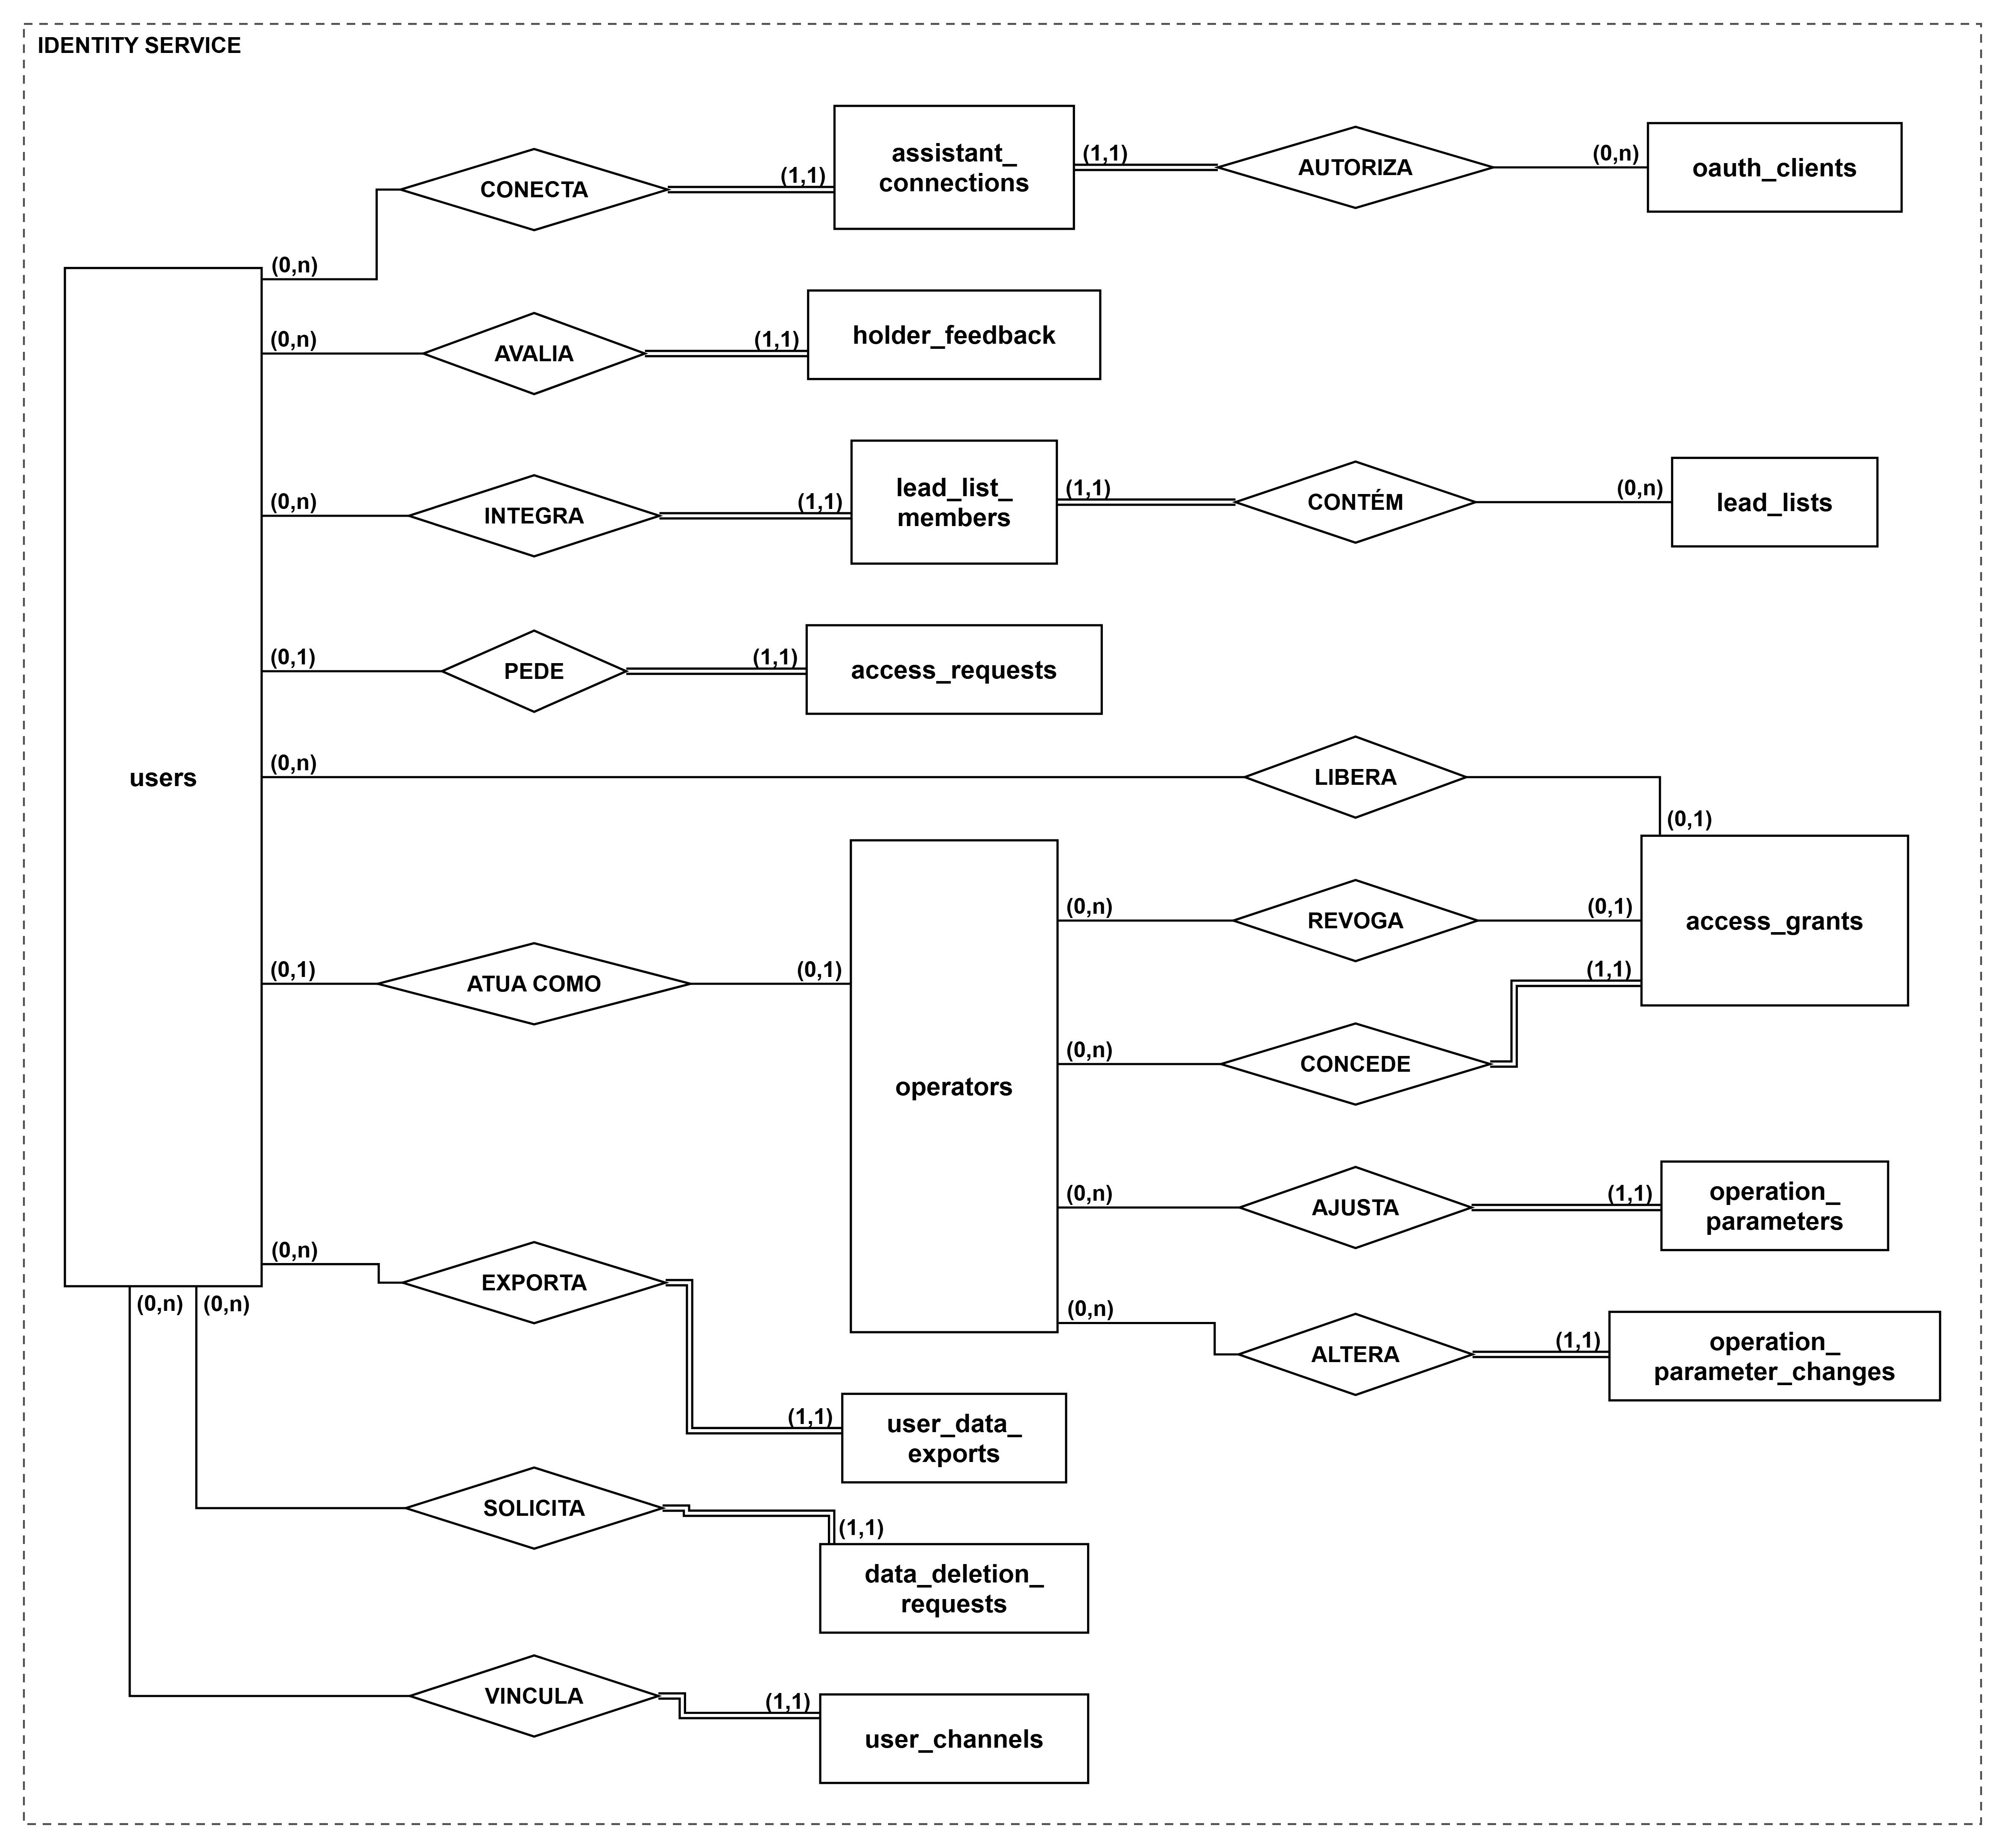
\includegraphics[width=\textwidth]{images/der_identity.png}
    \authorssource
\end{figure}

\begin{figure}[H]
    \centering
    \caption{DER do Finance Service}
    \label{fig:der_finance}
    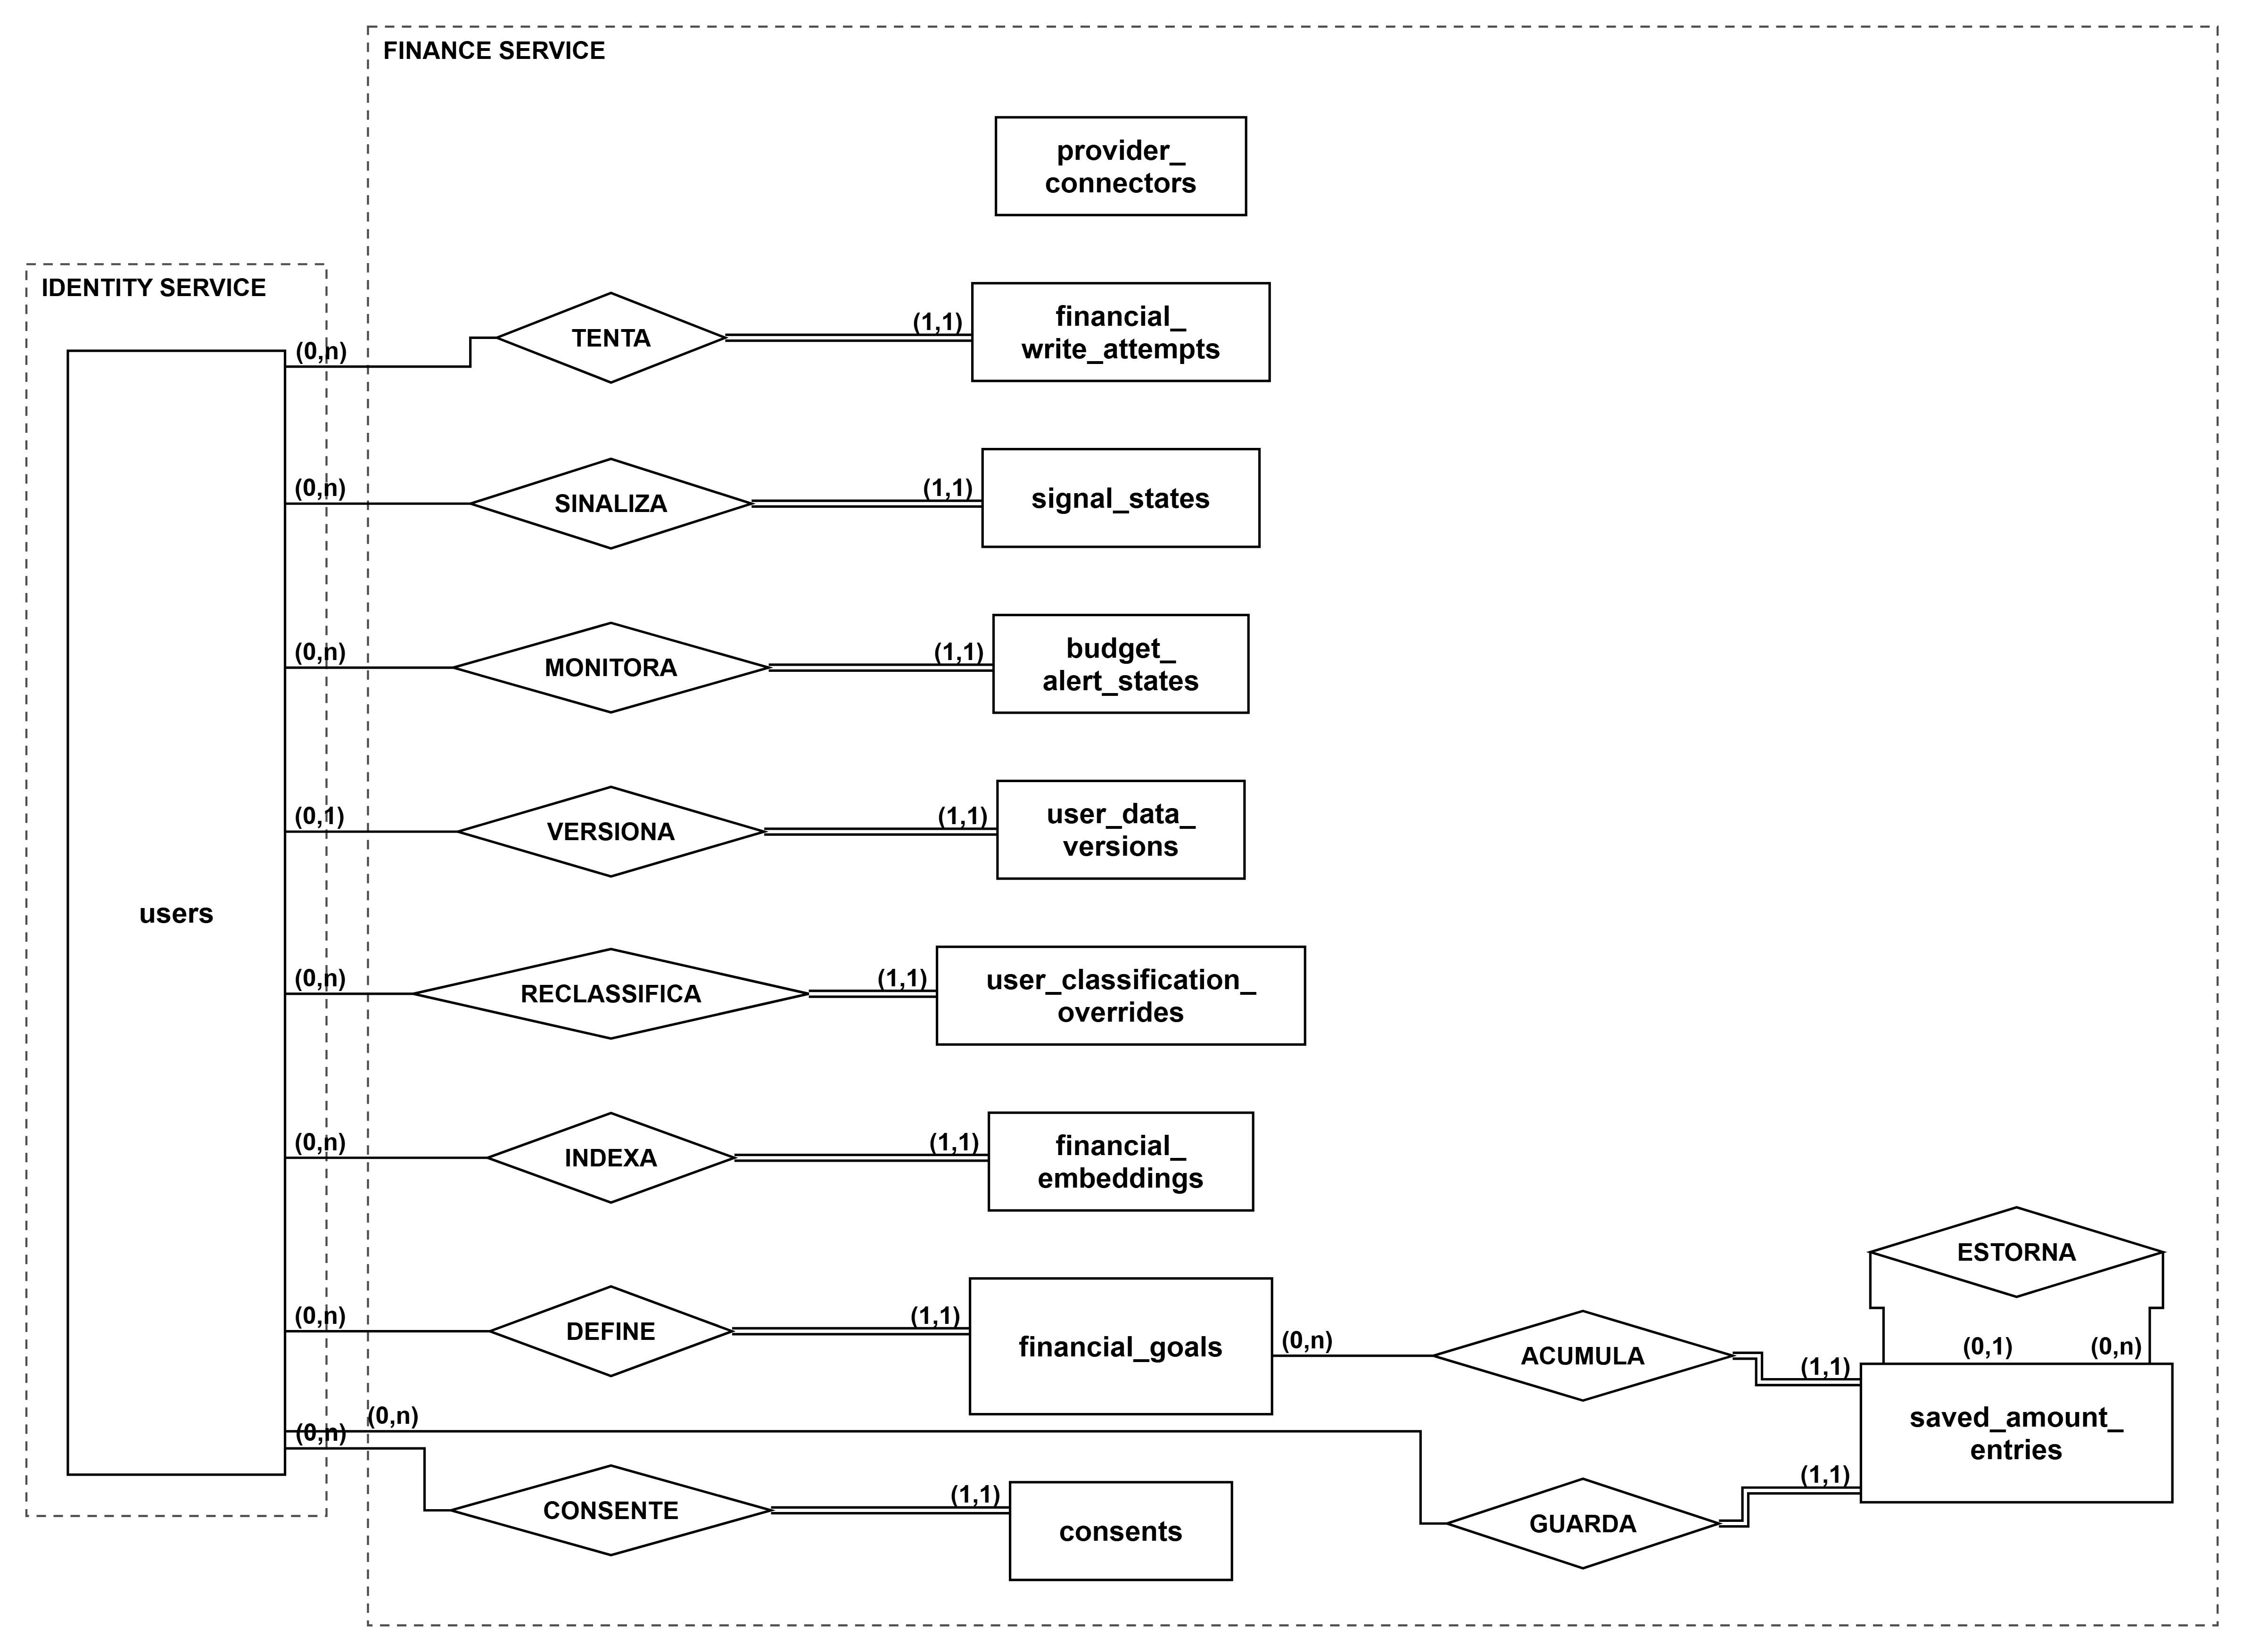
\includegraphics[width=\textwidth]{images/der_finance.png}
    \authorssource
\end{figure}

\begin{figure}[H]
    \centering
    \caption{DER do Billing Service}
    \label{fig:der_billing}
    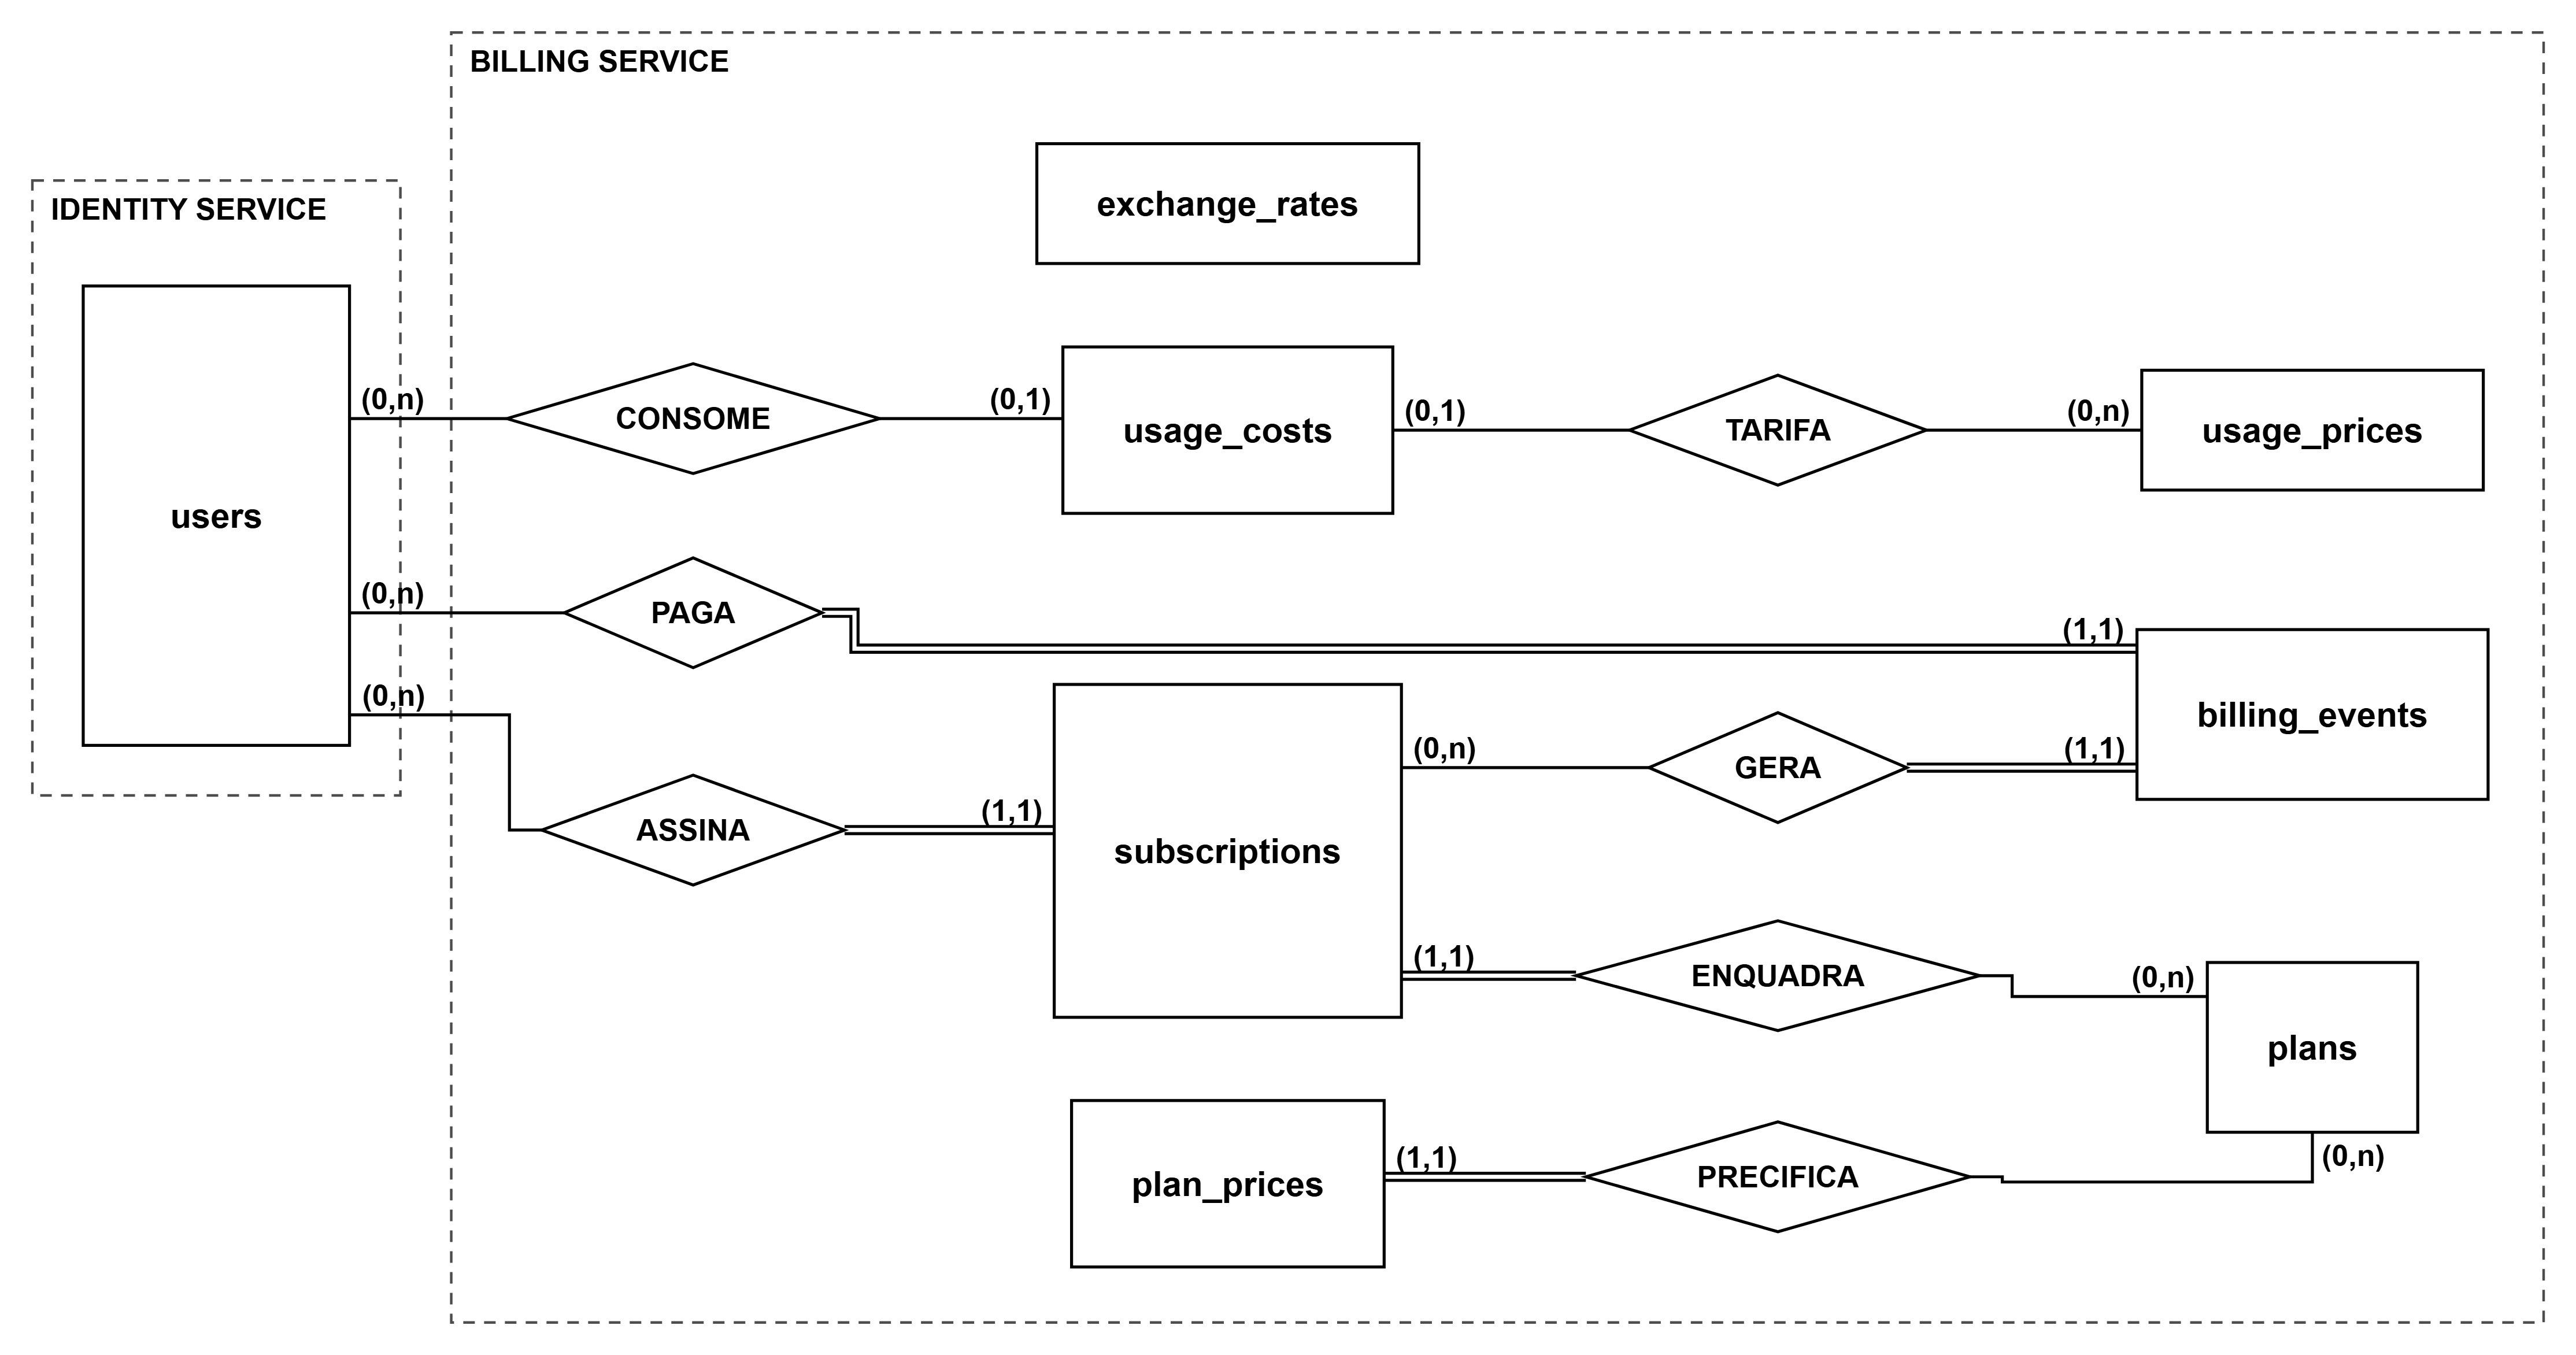
\includegraphics[width=\textwidth]{images/der_billing.png}
    \authorssource
\end{figure}

\begin{figure}[H]
    \centering
    \caption{DER do Notification Service e do Audit Service}
    \label{fig:der_notification}
    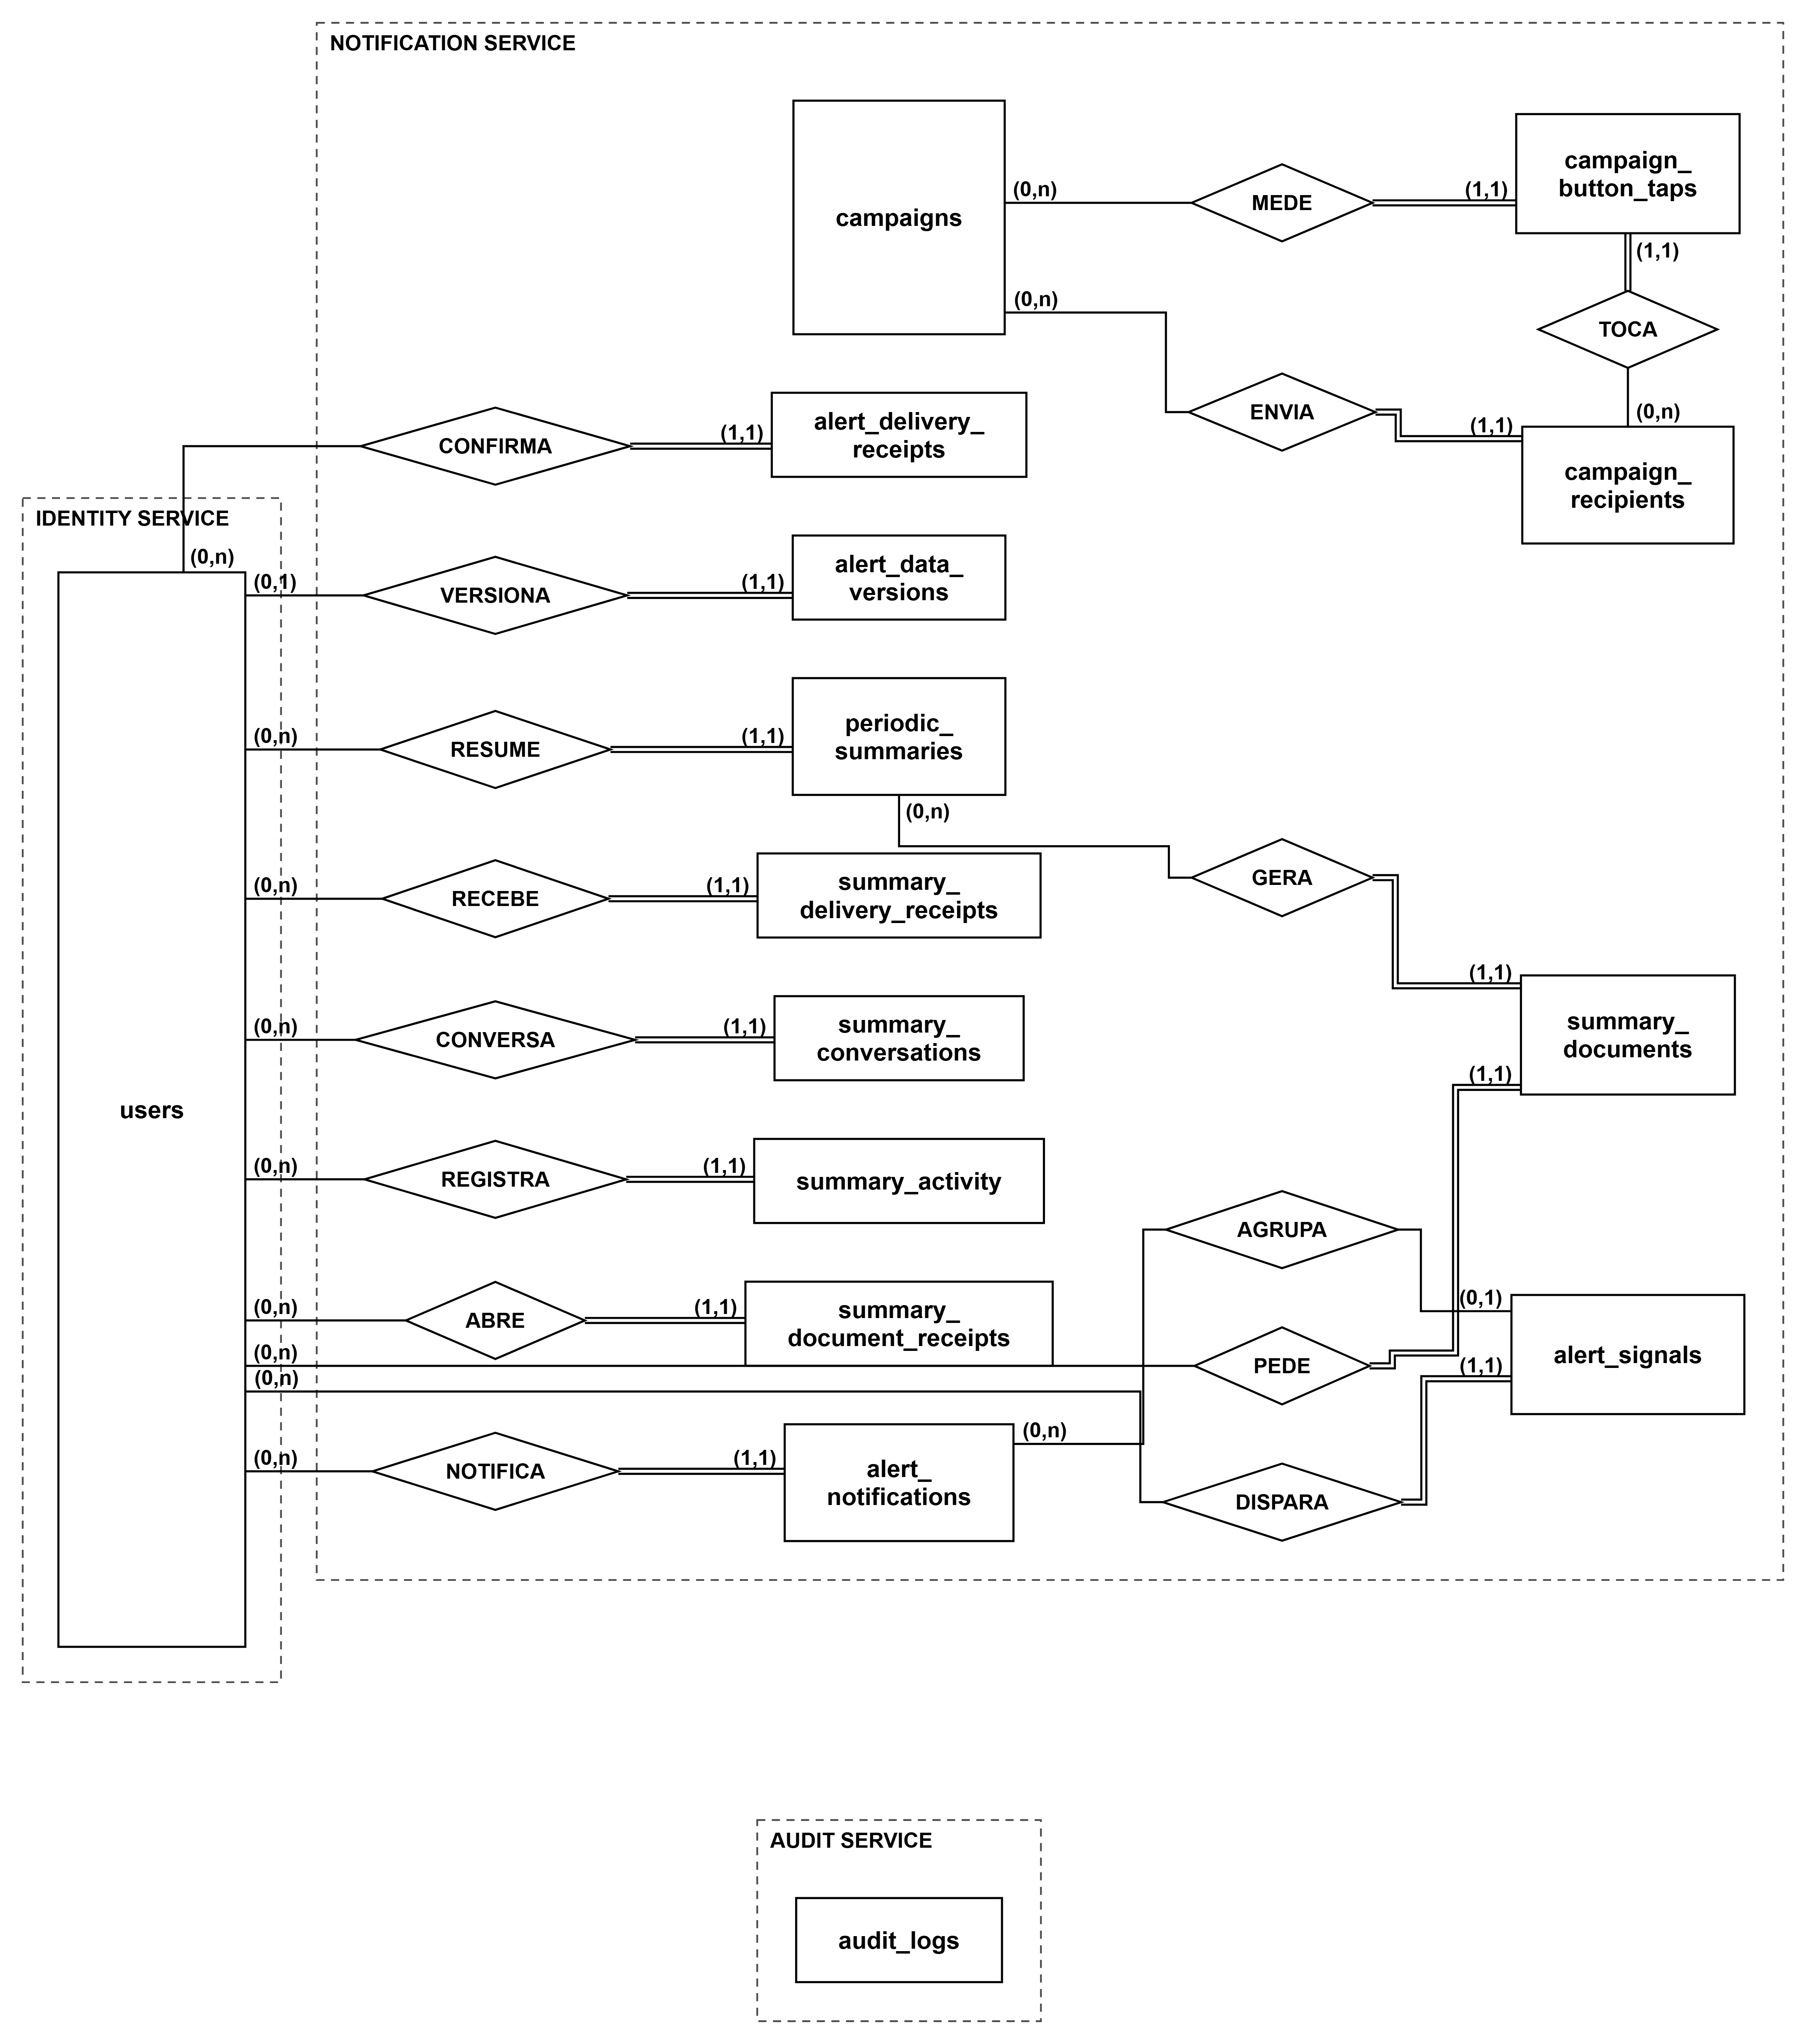
\includegraphics[width=\textwidth]{images/der_notification.png}
    \authorssource
\end{figure}

\section{Modelo lógico}

O Modelo Entidade-Relacionamento (MER), representado pelo DER das Figuras~\ref{fig:der_identity} a~\ref{fig:der_notification}, é empregado para representar os elementos do mundo real por meio de entidades, as quais possuem atributos que descrevem suas características, e relacionamentos que estabelecem conexões entre essas entidades (ELMASRI; NAVATHE, 2011). A partir do MER, deriva-se o modelo lógico, que representa as entidades como tabelas, com chaves primárias e estrangeiras e tipos de dados.

Na Figura~\ref{fig:mer_postgres} é apresentado o modelo lógico do núcleo do banco relacional, com os atributos principais do titular, das identidades de canal, dos consentimentos, das metas, das assinaturas, dos custos e dos pedidos relacionados à LGPD. As colunas com sufixo \texttt{\_encrypted} são cifradas com \texttt{pgcrypto} antes da gravação. As colunas \texttt{cpf\_hash} e \texttt{external\_id\_hash} guardam um HMAC-SHA256, isto é, um HMAC calculado com o algoritmo seguro de \textit{hash} (\textit{Secure Hash Algorithm}, SHA) de 256 bits, que permite a busca sem expor o valor original; a coluna \texttt{pin\_hash} guarda o PIN processado com o bcrypt, e as colunas \texttt{previous\_hash} e \texttt{record\_hash} encadeiam os registros de auditoria com o SHA-256. As tabelas de operação, campanhas, resumos e avisos seguem o mesmo padrão e estão representadas no DER.

\begin{figure}[H]
    \centering
    \caption{Modelo lógico do núcleo do sistema no PostgreSQL}
    \label{fig:mer_postgres}
    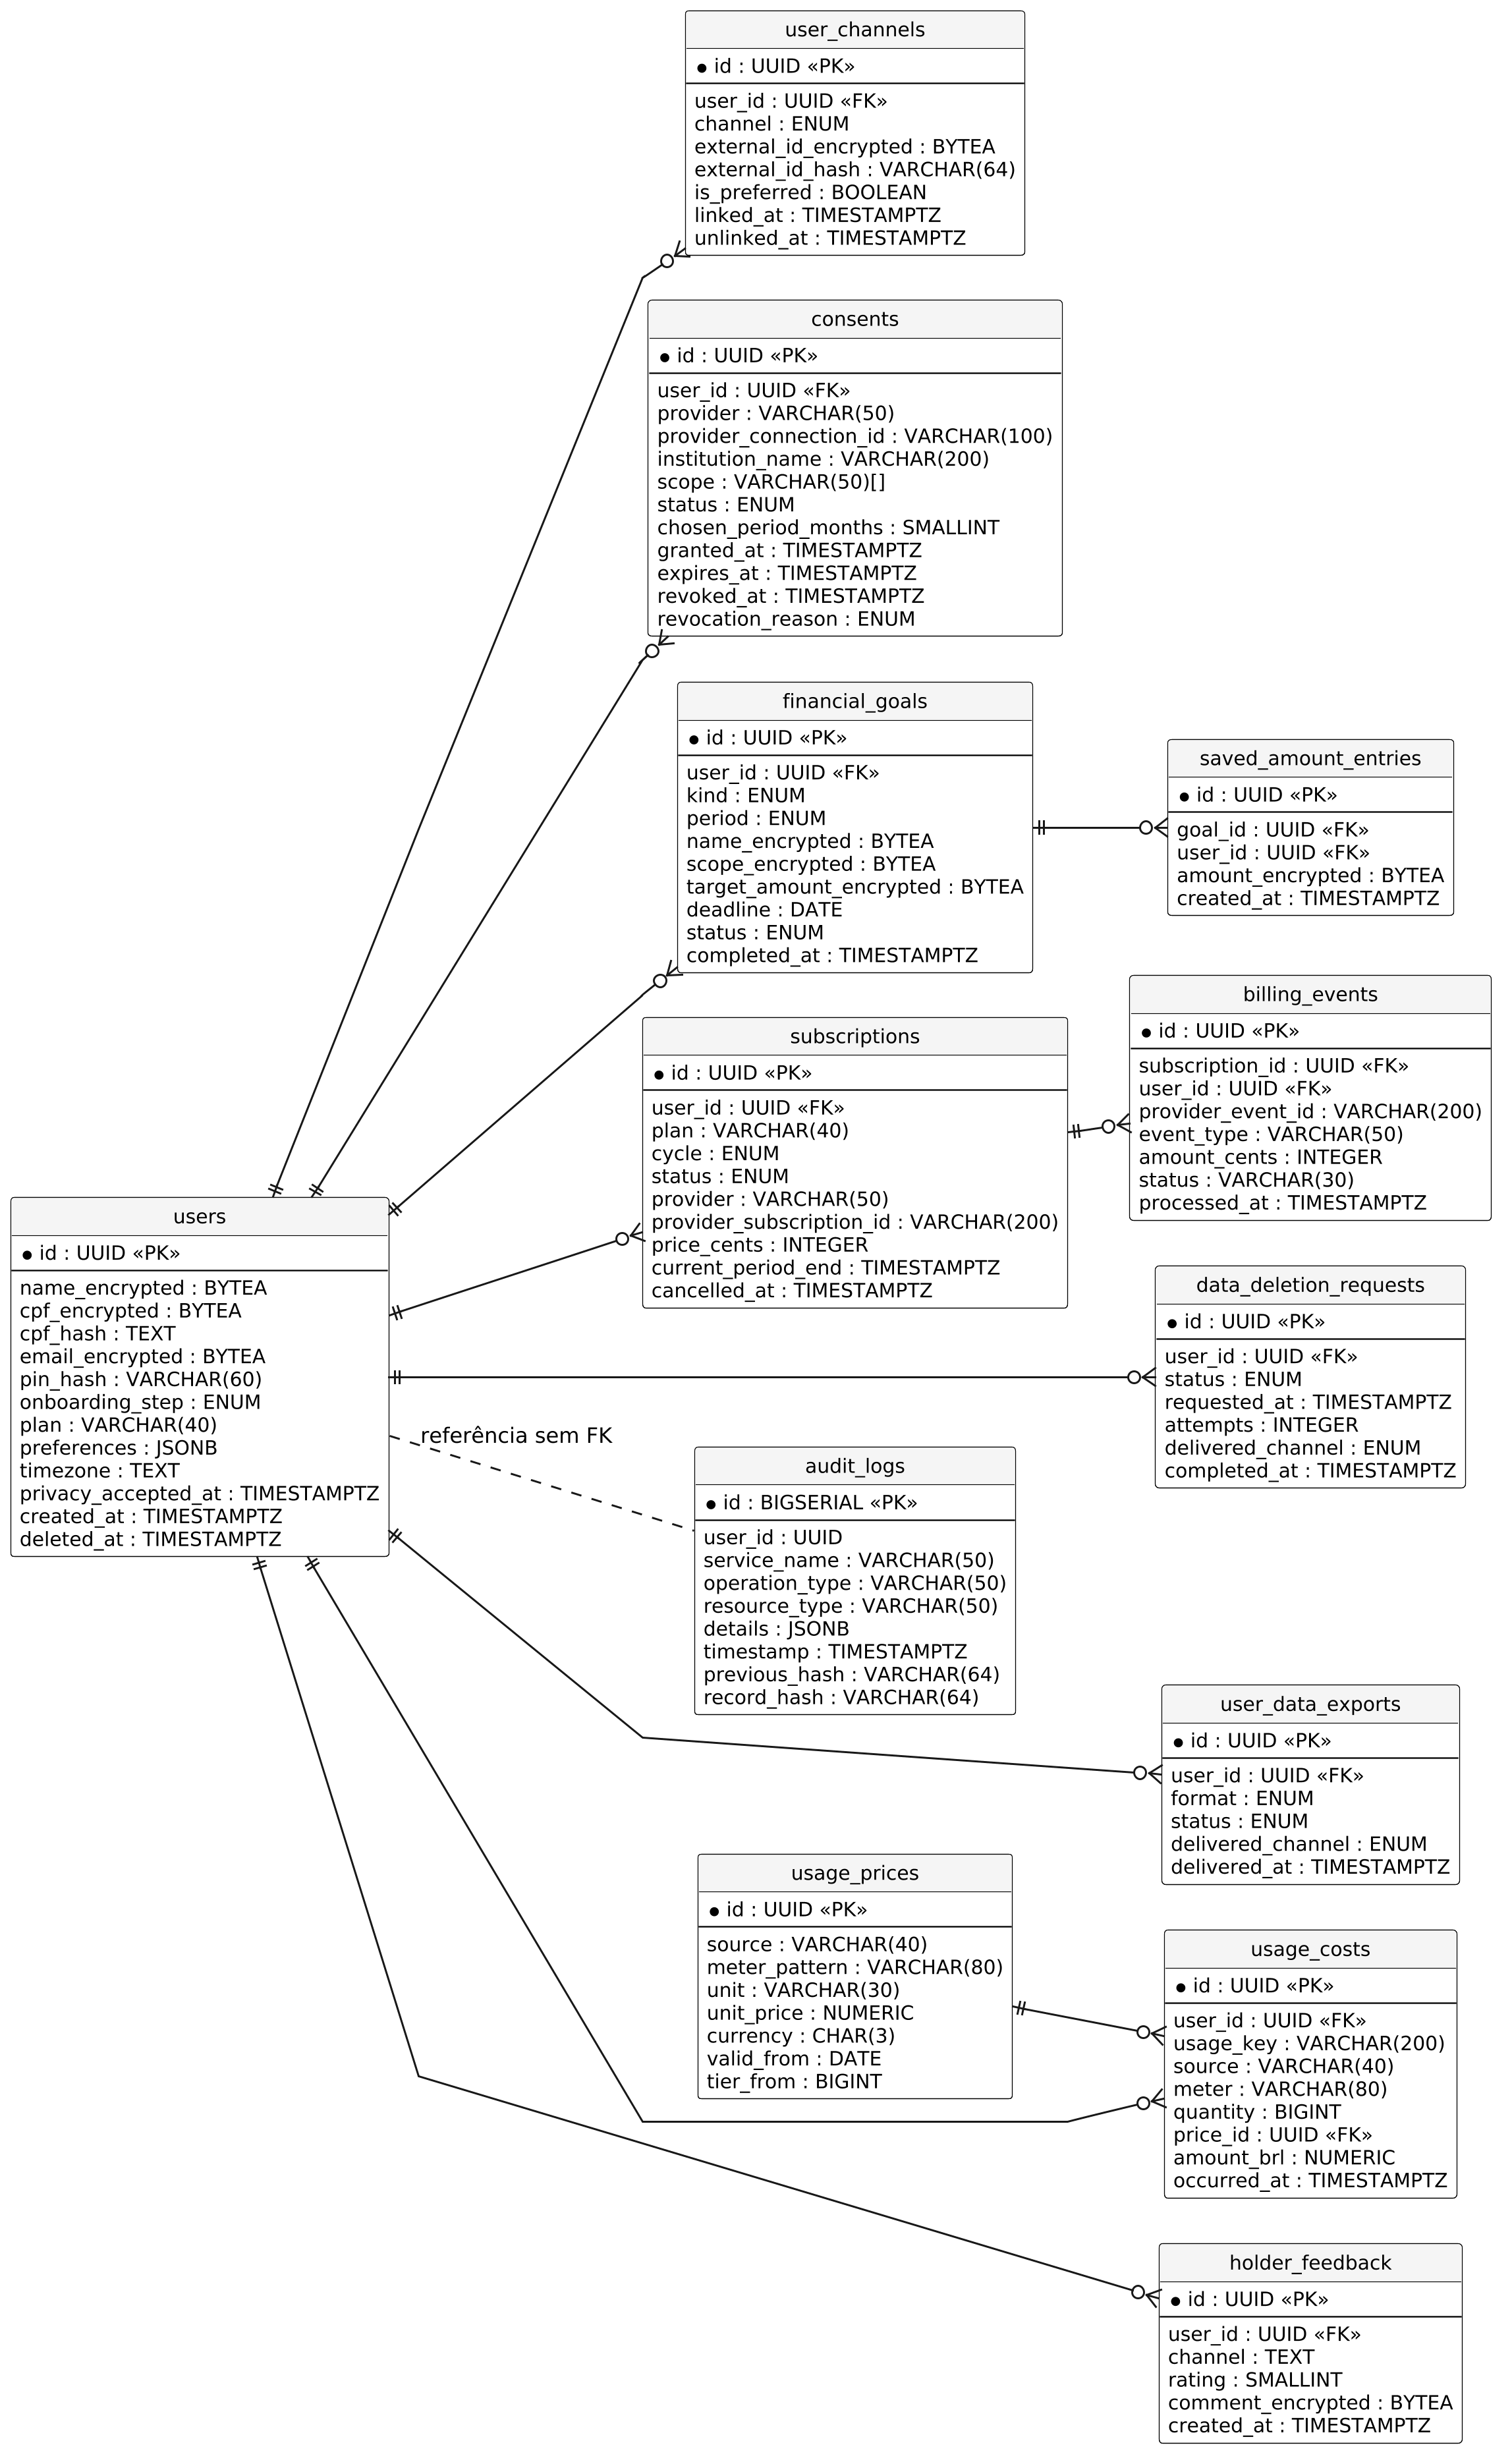
\includegraphics[width=\textwidth]{images/mer_postgres.png}
    \authorssource
\end{figure}

\section{Modelo de dados orientado a documentos}

O MongoDB, em um serviço gerenciado, armazena os dados sincronizados via Open Finance, o histórico de conversas dos usuários e as projeções calculadas pelo Analytics Service. A flexibilidade do modelo de documentos permite representar estruturas que variam conforme a instituição e o tipo de produto financeiro, sem a necessidade de migrações de esquema. Em atendimento à LGPD, campos monetários e textuais sensíveis são cifrados na camada de aplicação, antes da persistência, com o AES-256-GCM, isto é, o padrão de cifragem avançada (\textit{Advanced Encryption Standard}, AES) com chave de 256 bits no modo Galois/contador (\textit{Galois/Counter Mode}, GCM), com uma chave derivada para cada titular.

Na Figura~\ref{fig:mongo}, que apresenta o modelo de dados orientado a documentos utilizado no MongoDB, esses campos estão indicados como cifrados.

\begin{figure}[H]
    \centering
    \caption{Modelo de dados do MongoDB}
    \label{fig:mongo}
    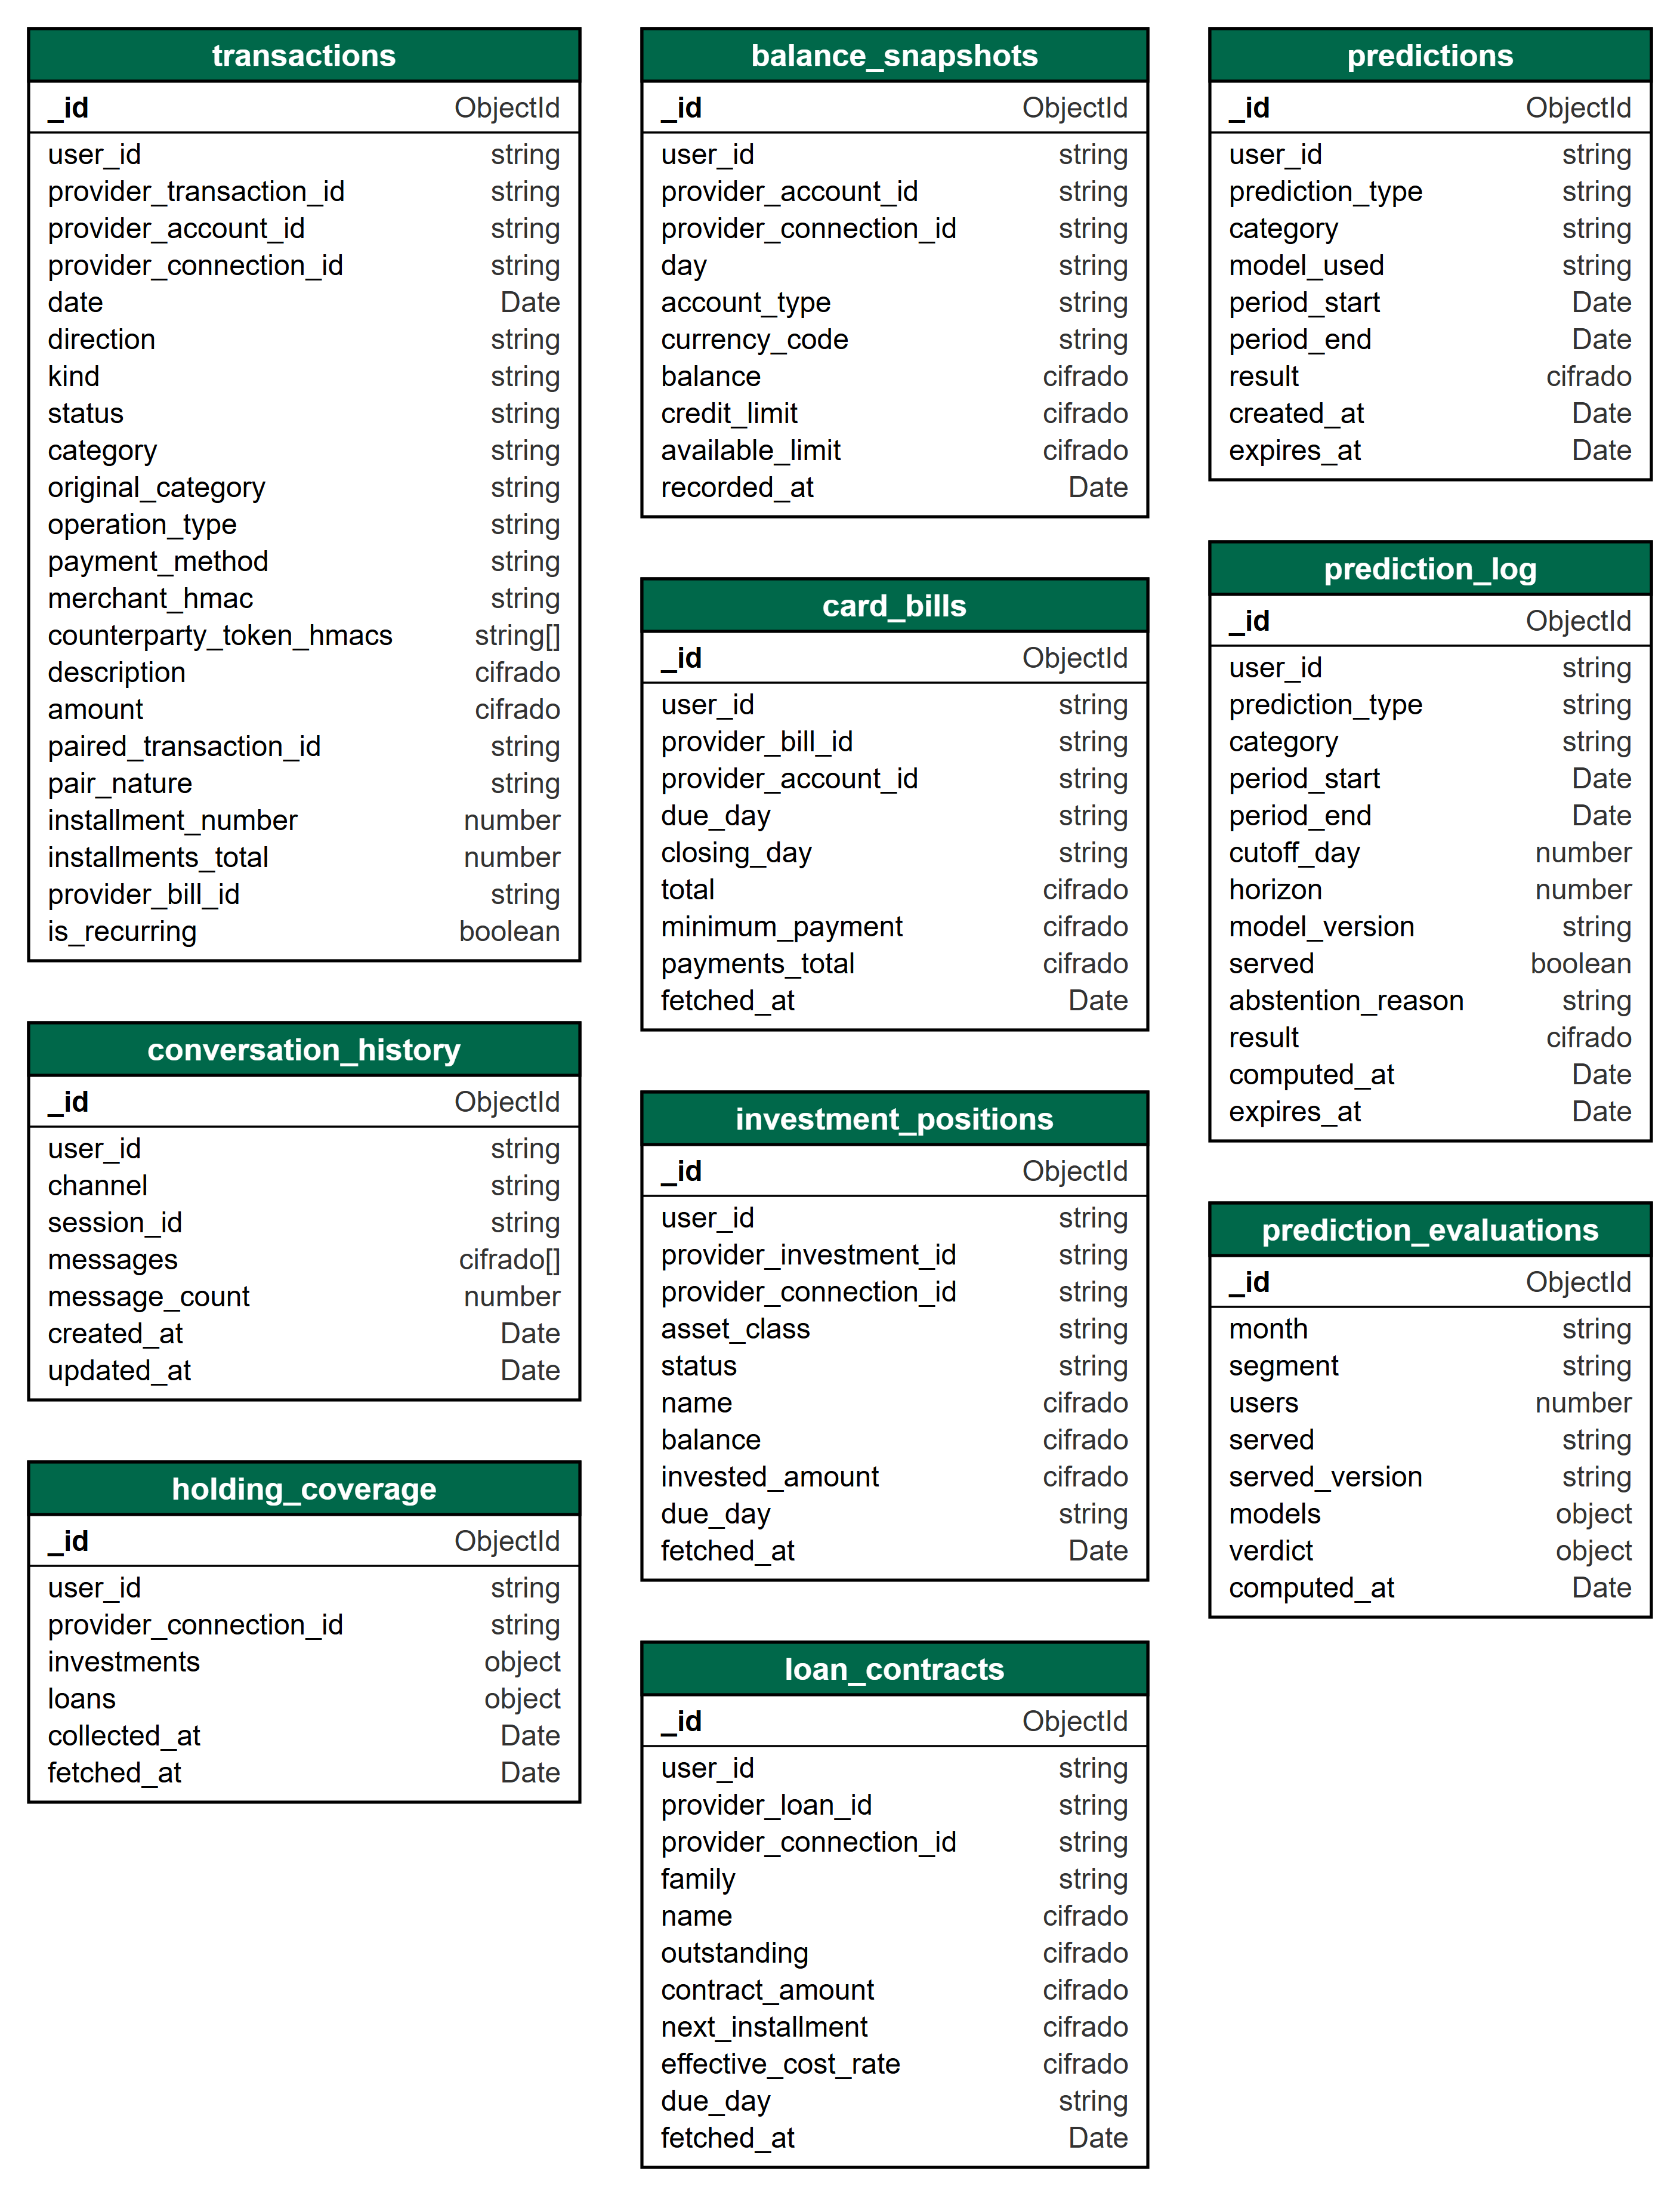
\includegraphics[width=\textwidth,height=0.8\textheight,keepaspectratio]{images/mongo.png}
    \authorssource
\end{figure}

O banco de dados MongoDB é organizado em dez coleções, descritas a seguir.

\subsection{Coleção \texttt{transactions}}

A coleção \texttt{transactions} armazena cada transação sincronizada a partir das instituições conectadas. O identificador da transação no agregador evita duplicidades em sincronizações subsequentes. Além da data, da categoria do sistema, do grupo dessa categoria, da categoria original informada pelo banco e da forma de pagamento, cada documento guarda a direção do dinheiro e a natureza do lançamento (consumo, movimentação entre contas, investimento, empréstimo, receita ou estorno), o que permite separar o que é gasto do que apenas mudou de lugar. Os dois lançamentos que registram um mesmo evento, como o pagamento de uma fatura, são ligados por \texttt{paired\_transaction\_id}. A descrição e o valor são cifrados, e a busca por estabelecimento usa HMACs da marca e de cada palavra do nome, sem guardar o nome em claro.

\subsection{Coleções de Saldos, Faturas, Investimentos e Empréstimos}

A coleção \texttt{balance\_snapshots} registra, por dia, o saldo de cada conta e o limite de cada cartão, o que permite acompanhar a evolução do patrimônio. A coleção \texttt{card\_bills} guarda as faturas de cartão, com vencimento, fechamento, total e pagamentos. As coleções \texttt{investment\_positions} e \texttt{loan\_contracts} guardam a última leitura dos investimentos e empréstimos informados pelo banco, e \texttt{holding\_coverage} registra o que cada instituição informa ou não, pois a ausência de um dado nem sempre significa que ele não existe. Os valores dessas coleções também são cifrados.

\subsection{Coleção \texttt{conversation\_history}}

A coleção \texttt{conversation\_history} persiste o histórico das conversas entre o usuário e o assistente, separado por canal e por sessão, o que permite retomar o contexto e responder a uma mensagem citada. Cada mensagem é cifrada com AES-256-GCM, e os segredos digitados na conversa, como PIN e CPF, são substituídos por um marcador antes da gravação. Um índice de tempo de vida (\textit{Time-to-Live}, TTL) de 90 dias exclui automaticamente os históricos antigos, em conformidade com o princípio de minimização de dados da LGPD.

\subsection{Coleções de Projeções}

A coleção \texttt{predictions} guarda as projeções calculadas pelo Analytics Service, com o método utilizado, o período e o resultado cifrado, incluindo a abstenção quando nenhum método é aprovado no teste retrospectivo. A coleção \texttt{prediction\_log} é o registro de previsões: acumula, a cada data de corte do mês, a estimativa do método em uso, exibida ao titular, e a dos candidatos calculados em paralelo, sem exibição ao titular, nos segmentos de gasto do mês, dos meses seguintes e de saldo livre, também com os valores cifrados. A coleção \texttt{prediction\_evaluations} guarda o fechamento mensal, que compara cada registro com o valor que de fato ocorreu e grava, por segmento, as medidas de cada candidato e a decisão que pode liberar ou desativar um método. Os documentos de \texttt{predictions} e de \texttt{prediction\_log} expiram automaticamente.
